\documentclass[10pt,technote]{IEEEtran}
\usepackage{amssymb}
\usepackage{amsmath}
\usepackage{graphicx}
\usepackage{subcaption}
\title{Coursework 1: Face recognition }
\author{Timothee Gathmann, Luka Lagator}
\begin{document}

\maketitle


\section{Question 1}
\subsection{Eigenfaces}
\subsubsection{Part a)}
The faces dataset consisted of 10 pictures for each of the 52 different individuals. Hence, it was decided to split the data into 7 pictures per individual for training and 3 pictures per individual for testing, resulting in a total of 364 training images. This allowed to train the PCA algorithm on all available classes and run meaningful tests on all images. Moreover, the order of pictures per individual was randomised before to remove any possible correlation between the complexity/characteristics of the pictures and their order, hinted by previous experiments. We found that with the added random component, overall, the classification accuracy improved from the initial experiments where first 7  pictures per individual were taken as the training set.

Standard PCA was performed and the eigenfaces in Figure \ref{fig:eigfaces1} were found, along with the eigenvalues in Figure \ref{fig:eigvals1}. The data was normalised by subtracting the mean face shown in Figure \ref{fig:mean_im1}. In order to identify relevant principal components, the eigenvalues of the covariance matrix with a real part lower than 0.1 were discarded (the number was chosen by inspection). 363 ($N - 1$) eigenfaces and eigenvalues remained after this thresholding operation, meaning that 363 eigenfaces were relevant to optimally reduce the dimensionality of the data. Notably, for $N$ training samples, the number of relevant eigenvalues was found to be $N - 1$. This is expected, since the mean image is removed, the largest vector subspace that can be defined with N points is $R^{N-1}$.
% How do you choose how many eigenvectors you'll actually keep ?
The eigenfaces (eigenvectors) with larger eigenvalues represent the most varied features of the training images (or the projection directions with the largest data scatter). Hence, the eigenvectors with larger eigenvalues will be more important for NN classification.
The plot of accuracy vs the number of retained eigenfaces is shown in Figure \ref{fig:how_many_faces}. We can see the accuracy improves significantly at first and then less with addition of the less important eigenfaces, which is what we expect.
\begin{figure}[htb!]
    \centering
    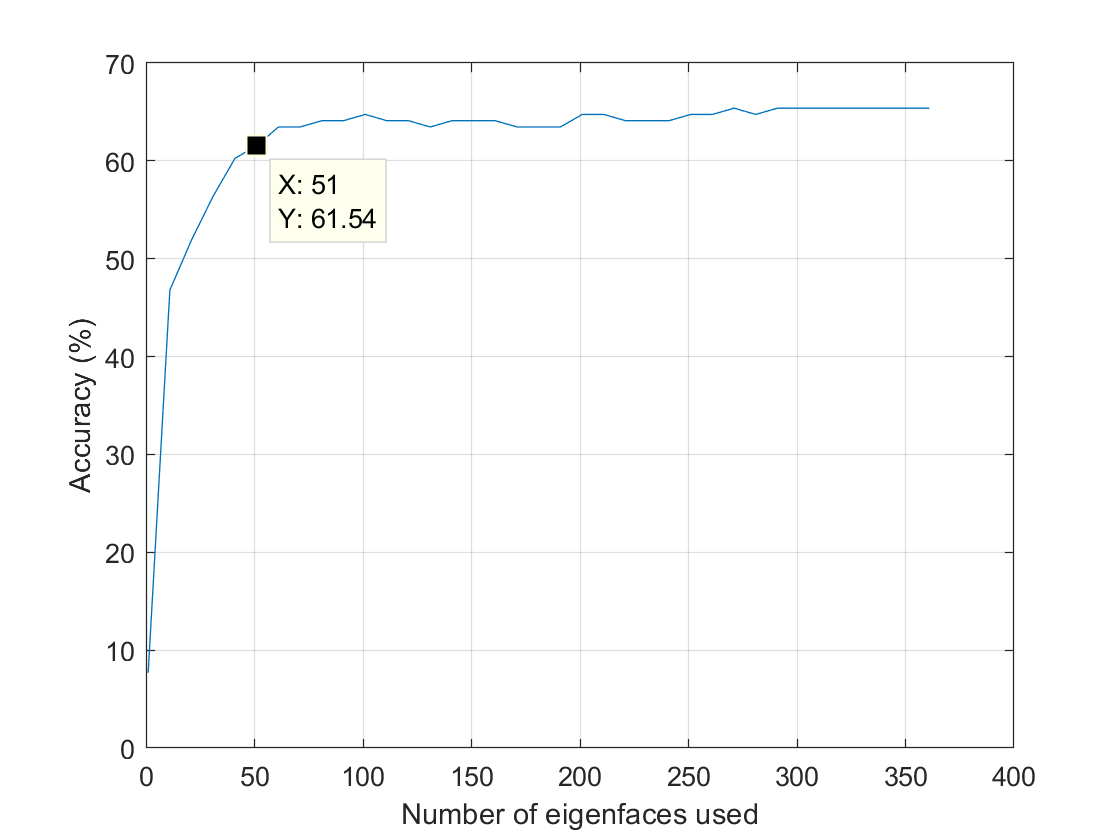
\includegraphics[width=\linewidth]{../results/1bb/how_many_eigenfaces.png}
    \caption{Classification accuracy by NN against number of eigenfaces. 52 eigenfaces give a satisfactory result}
    \label{fig:how_many_faces}

\end{figure}

\begin{figure}[htb!]
    \centering
    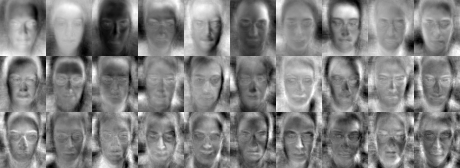
\includegraphics[width=0.4\textwidth]{../results/ex1a/eigenfaces.png}
    \caption{Eigenfaces with the 30 largest eigenvalues}
    \label{fig:eigfaces1}
\end{figure}

\begin{figure}[htb!]
    \centering
    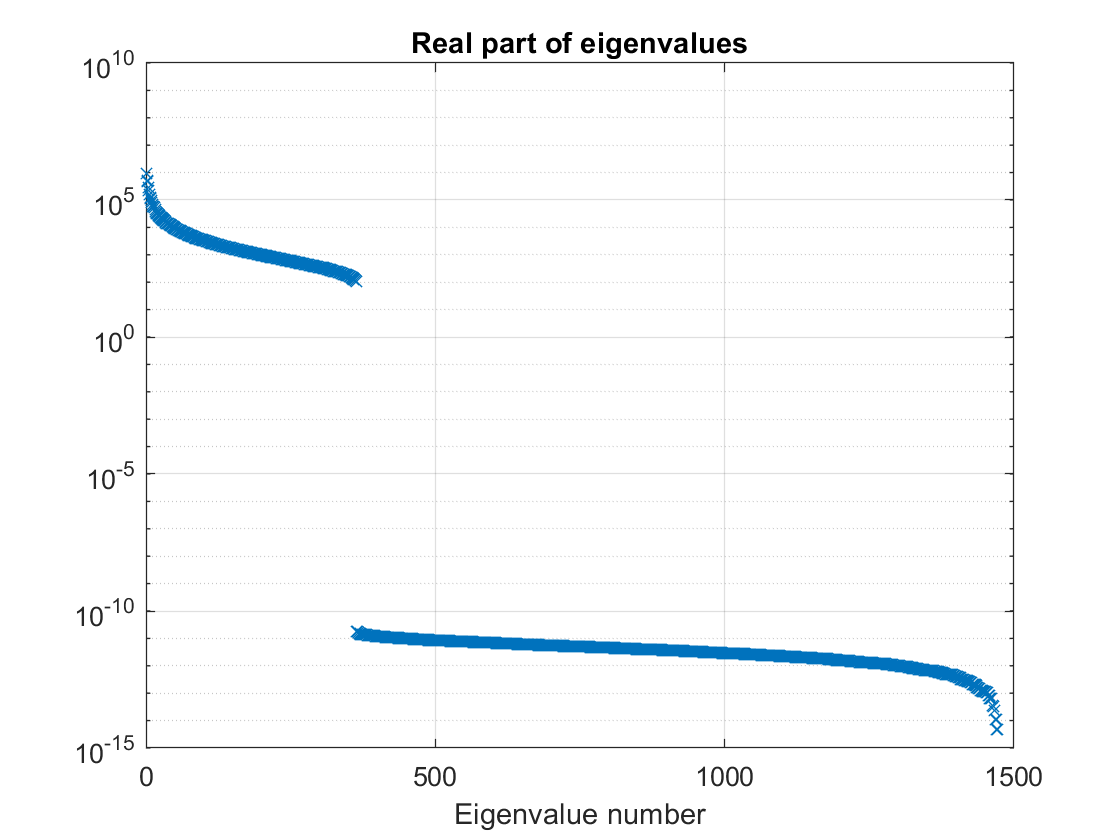
\includegraphics[width=0.4\textwidth]{../results/ex1a/eigenvalues.png}
    \caption{Real part of all PCA eigenvalues (semi-log-y axis). Negative eigenvalues were discarded but were close to 0.}
    \label{fig:eigvals1}
\end{figure}

\begin{figure}[htb!]
    \centering
    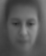
\includegraphics[width=0.1\textwidth]{../results/ex1a/mean_image.png}
    \caption{Mean image of the training dataset}
    \label{fig:mean_im1}
\end{figure}

\subsubsection{Part b)}
The low-dimensional computation returns, as expected, $N - 1$ eigenvalues and eigenvectors which we then compare to the original ones from Part b) in Figure \ref{fig:eig_diff1}. We can notice that there is no difference between the eigenvalues obtained from high-dimensional and low-dimensional computation. We also compare the eigenvectors' directions by normalising them and taking their dot product (cosine similarity). We can see in the bottom plot that the new eigenvectors have the same direction as before. 
The low-dimensional computation proved to be 72 times faster than the standard computation, even though it involved more steps, since the dimensionality of the matrix from which the eigenvectors were computed was lower.
% What's a con of this method ? Vector normalization?
\begin{figure}[htb!]
    \centering
    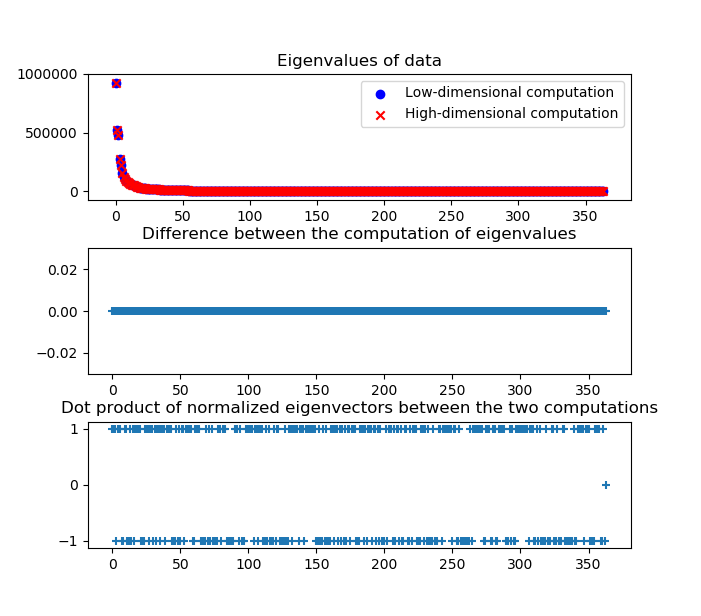
\includegraphics[width=\linewidth]{../results/ex1b/DIfference_eig.png}
    \caption{Comparison of the high-dimensional and low-dimensional computations of eigenvalues and eigenvectors. Negative dot product values indicate exactly opposed vectors.}
    \label{fig:eig_diff1}
\end{figure}

\subsection{Application of eigenfaces}
\subsubsection{Part a)}
The training data was used to find the eigenfaces. The testing data was projected in the PCA subspace, and it was attempted to reconstruct the test images as the number of retained eigenfaces was increased (until $N - 1$).

Quantitatively, the distortion (reconstruction error) is ever decreasing as the number of eigenvectors used for reconstruction increases, as shown in Figure \ref{fig:distortion}. However, the improvement gets slower as the number of eigenvectors increases, hinting that the full number of eigenvectors is not necessary to achieve a 'good-enough' reconstruction. As expected, when the full number of eigenvectors ($N - 1$) is used, the reconstruction is perfect (distortion of the order of $10^{-19}$)

This shows qualitatively in Figure \ref{fig:reconstr_faces}: the faces get reliably recognisable with around $M =150$ eigenvectors, whereas complex shadowing details appear only when more eigenfaces are used.
\begin{figure}[htb!]
    \centering
    \begin{subfigure}[b]{\linewidth}
        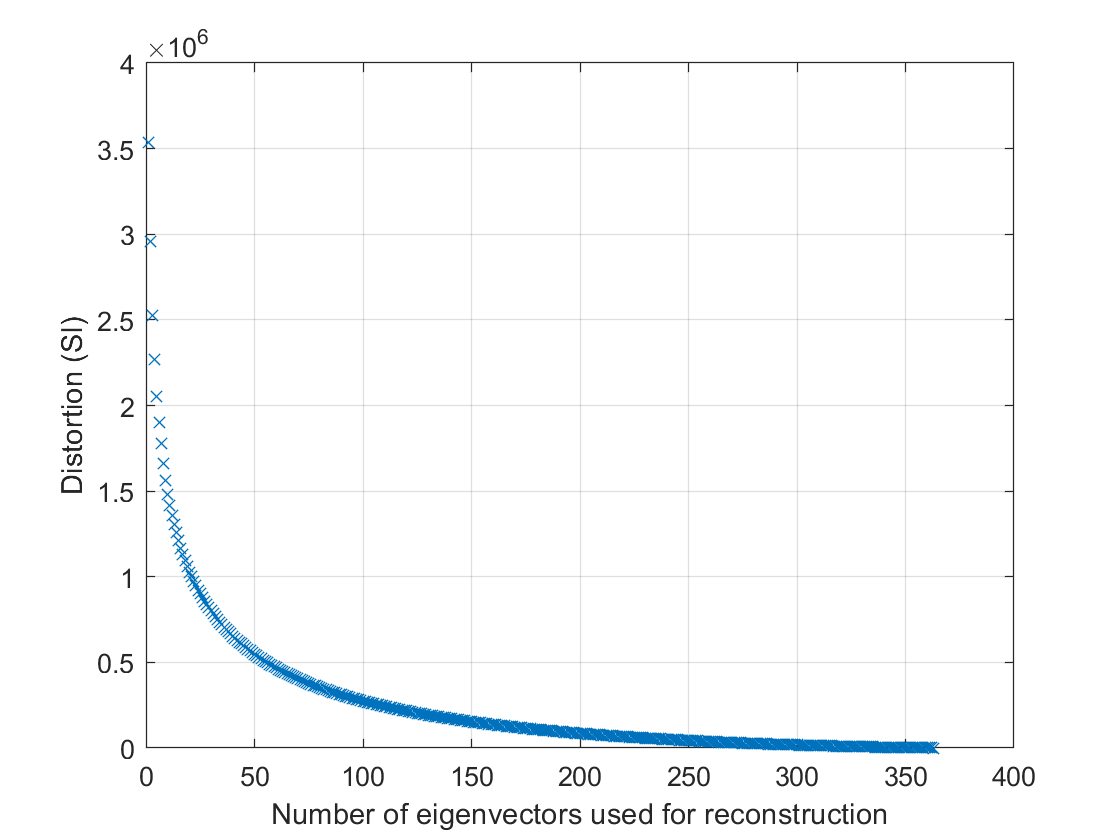
\includegraphics[width=\textwidth]{../results/ex1aa/dist_plot.png}
        \caption{Normal scale}
        
        \quad
    \end{subfigure}
    \begin{subfigure}[b]{\linewidth}
        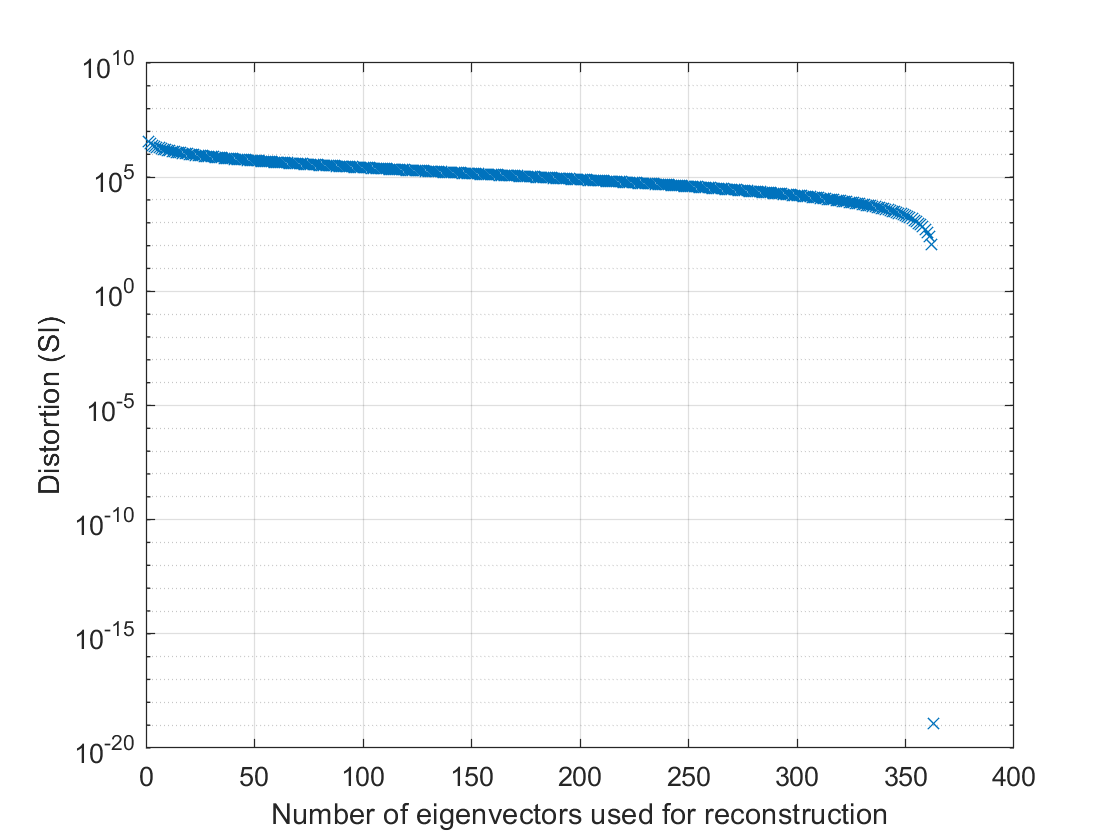
\includegraphics[width=\textwidth]{../results/ex1aa/dist_logplot.png}
        \caption{Y axis in log scale}
        
        \quad
    \end{subfigure}
    \caption{Distortion of the reconstructed images when varying the number of eigenvectors used}
    \label{fig:distortion}
\end{figure}
\begin{figure}[htb!]
    \centering
    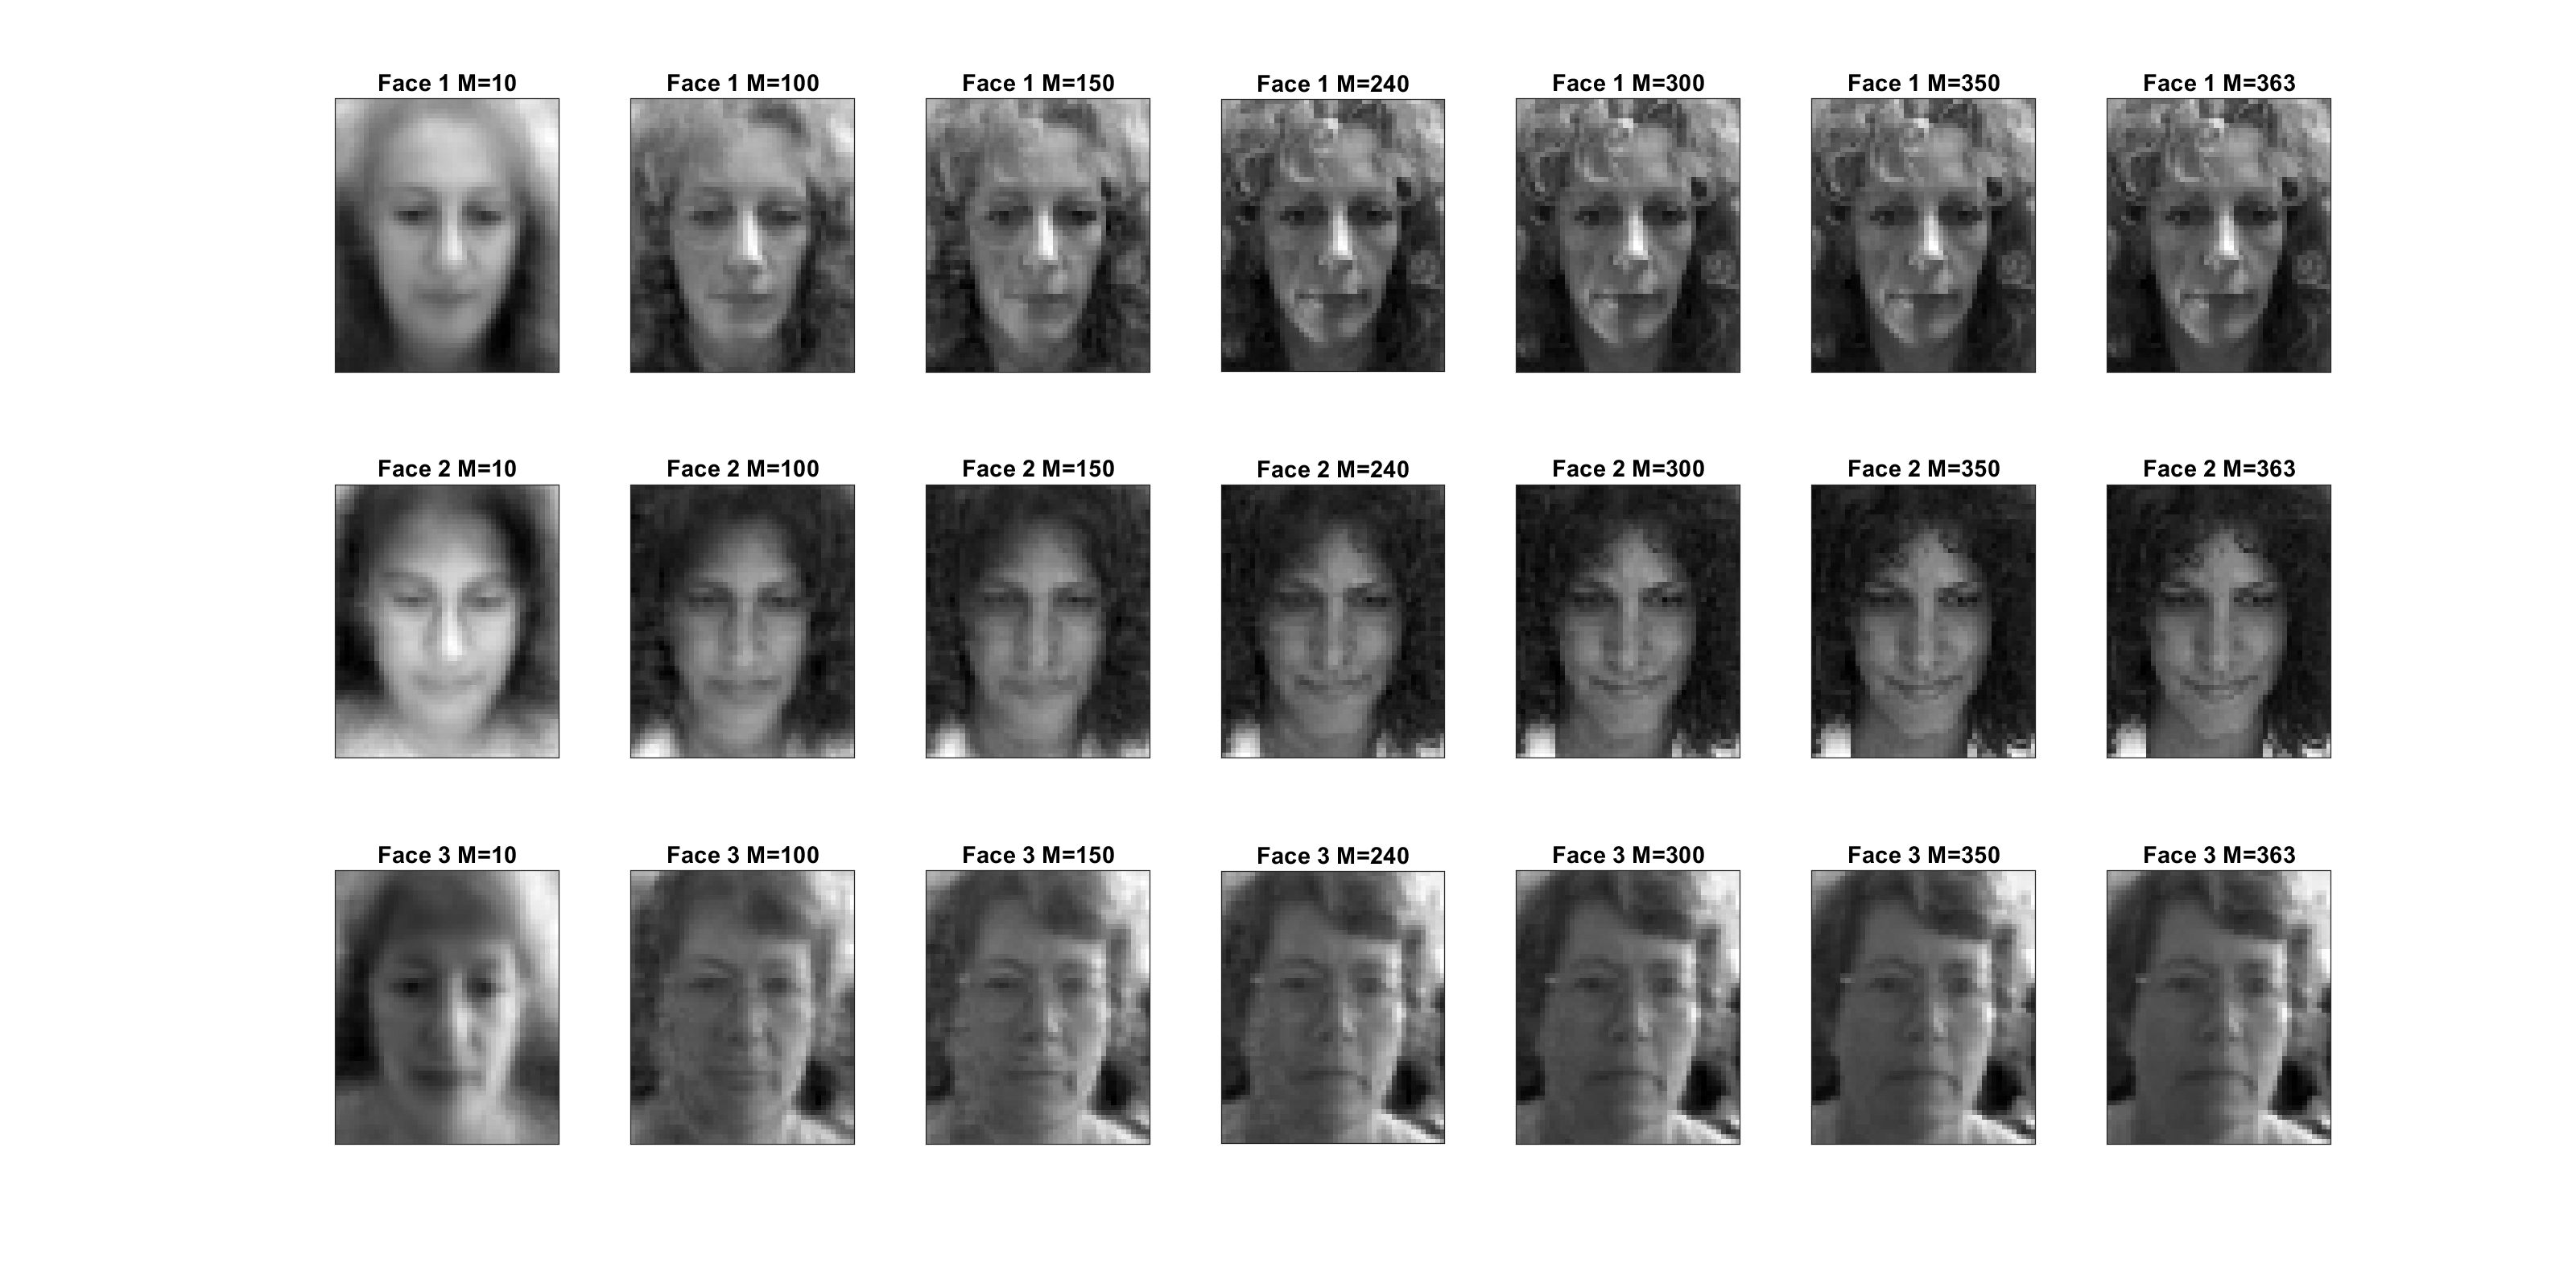
\includegraphics[width=\linewidth]{../results/ex1aa/face_plots.png}
    \caption{Reconstructed faces, M indicates the number of eigenvectors used}
    \label{fig:reconstr_faces}
\end{figure}


\subsubsection{Part b)}
Here we compare the performance of our model with two different classification methods. The Near Neighbour (NN) classification assigns the class of the nearest reference coefficient for each test image projected onto the PCA subspace. In classification by reconstruction, we first learn a different PCA subspace for each class (trained on images belonging to the class) and then project the test image onto each classes subspace. We then obtain 52 reconstructed images using the coefficients obtained from each class and finally assign the class with minimum reconstruction error when compared to the test image.
Table \ref{tab:NNvsRec} shows the difference between the two classification methods in terms of accuracy, classification time and memory usage.
Figures 7-10 show example success and failure cases for both methods of classification. Figures 11 and 12 show the confusion matrices for NN classification and classification by reconstruction respectively.
Both confusion matrices show a tendency to miss-classify the test images as particular classes. These particular classes(persons) seem to share similar features to many others. In this case the reconstruction method appears to perform worse. By learning a different subspace for each class, classes that share similar features (eigenfaces) produce similar coefficients and reconstruction errors, where these coefficients are weighted and summed (reinforcing class similarity). Conversely, the NN classification assigns nearest reference coefficient's class, regardless of the distance to other coefficients belonging to the class, and this seems to perform better when coefficients of two classes reside in close proximity to each other in the PCA subspace.

\begin{table}[]
    \centering
    \begin{tabular}{c||c c}
         & NN method & Reconstruction method  \\\hline \hline\\
         Accuracy &  69.2 \% & 55.8 \% \\
         Duration of classification & 0.332 s & 0.965 s \\
         Peak memory usage & 104.7 MiB & 94.7 MiB
         
    \end{tabular}
    \caption{Performance comparison of face recognition using the NN method and the reconstruction method}
    \label{tab:NNvsRec}
\end{table}



\begin{figure}[htb!]
    \centering
    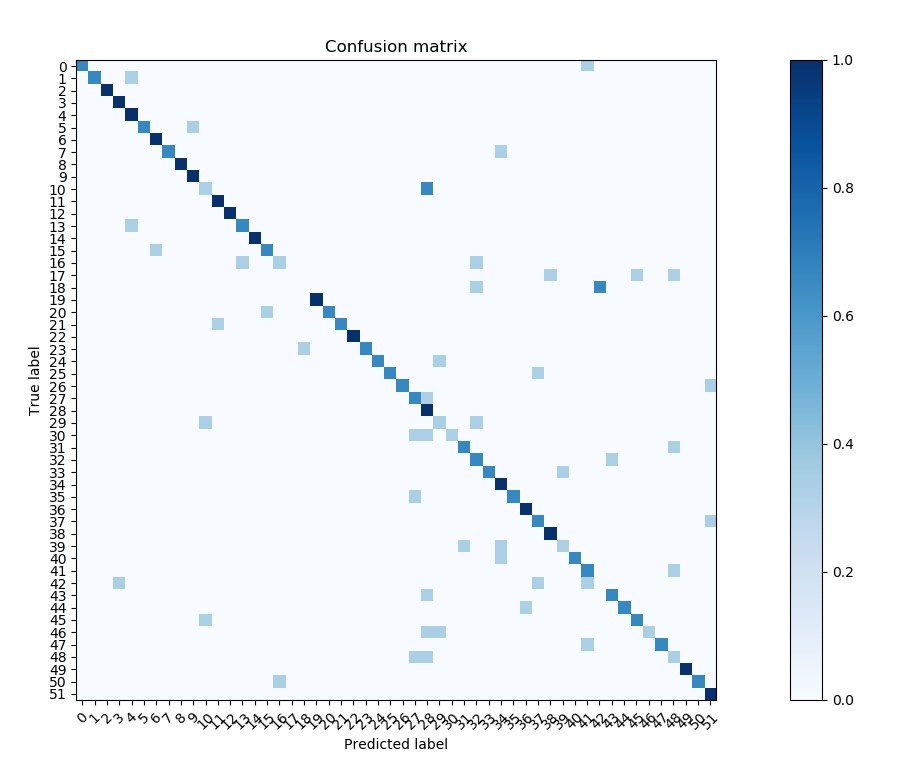
\includegraphics[width=\linewidth]{../results/1bb/confusion_NN.png}
    \caption{NN Classification Confusion Matrix}
    \label{fig:NN_conf_mat}
\end{figure}

\begin{figure}[htb!]
    \centering
    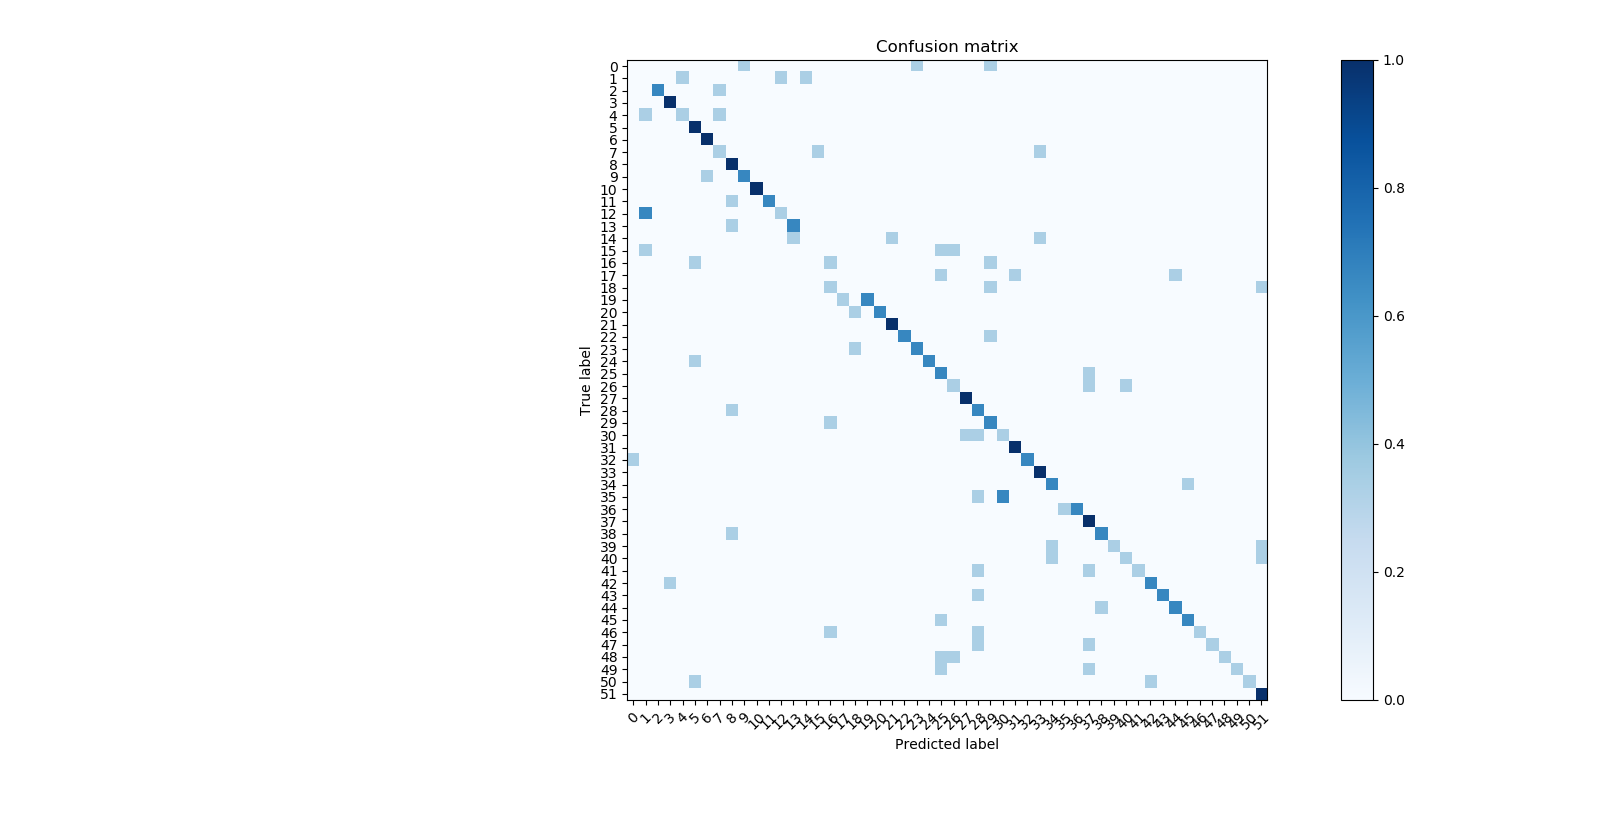
\includegraphics[width=\linewidth]{../results/1bb/confusion_rec.png}
    \caption{Classification by Reconstruction Confusion Matrix}
    \label{fig:REC_conf_mat}
\end{figure}

\section{Question 2}

PCA and LDA are opposed by their nature. The generative characteristic of PCA is achieved by maximising the scatter of all, unlabelled data-points ($S_T$). On the other hand, the discriminative characteristic of LDA is achieved by maximising the scatter between data points of different labels ($S_B$), and keeping the scatter within a class ($S_W$) constant. Hence, the goals of each of them are diametrically opposed and cannot be satisfied simultaneously.

Looking at the LDA criterion function:
\begin{equation}
    J(\boldsymbol{W_{LDA}}) = \frac{\boldsymbol{W_{LDA}}^T\boldsymbol{S}_B\boldsymbol{W_{LDA}}}{\boldsymbol{W_{LDA}}^T\boldsymbol{S}_W\boldsymbol{W_{LDA}}}
\end{equation}
Which we seek to maximise, while for PCA:
\begin{equation}
    J(\boldsymbol{W_{PCA}}) = |\boldsymbol{W_{PCA}}^T\boldsymbol{S}_T\boldsymbol{W_{PCA}}|
\end{equation}
Which we also which to maximise
Notably, maximising $S_T$ results in maximising $S_W$ and $S_B$ as a consequence, due to their intrinsic definition.

However, one way a trade-off could be achieved would be by finding a middle ground during the optimisation procedure. We can maximise the criterion 
\begin{equation}
    J(\boldsymbol{W_{opt}}) = \frac{\boldsymbol{W}^T(\alpha\boldsymbol{S}_T + (1 - \alpha)\boldsymbol{S}_B)\boldsymbol{W}}{\boldsymbol{W}^T\boldsymbol{S}_W\boldsymbol{W}}
\end{equation}
with $0 \le \alpha \le 1$, a parameter that would control the trade-off between both scatter matrices. A high value of alpha would encourage the generative side of our $W_{opt}$ while a low value would encourage its discriminative side. 
The optimisation procedure then follows in the same steps as in the slides, using a Lagrangian multiplier to keep the denominator constant.


\section{Question 3}
\subsection{PCA-LDA}
The data was split the same way for PCA-LDA algorithm training, with 70\% used for training and the rest for testing. 

\subsubsection{Recognition accuracy}
The top plot of Figure \ref{fig:mod_params_vs_acc} shows the results of  the experiment where the number of retained fisher-faces ($M_{lda}$) is gradually decreased, and the dimension of the PCA subspace ($M_{pca}$) is kept as N-c. We can see that the recognition accuracy worsens as the $M_{lda}$ decreases.

In the bottom plot we can see results of decreasing $M_{pca}$ while retaining all the fisherfaces ($c-1$). Our results show no particular trend in decreased classification accuracy. This supports the fact that we can learn much better features when applying discriminative, supervised algorithm, making the model more successful in classifying sparse features.

\begin{figure}
    \centering
    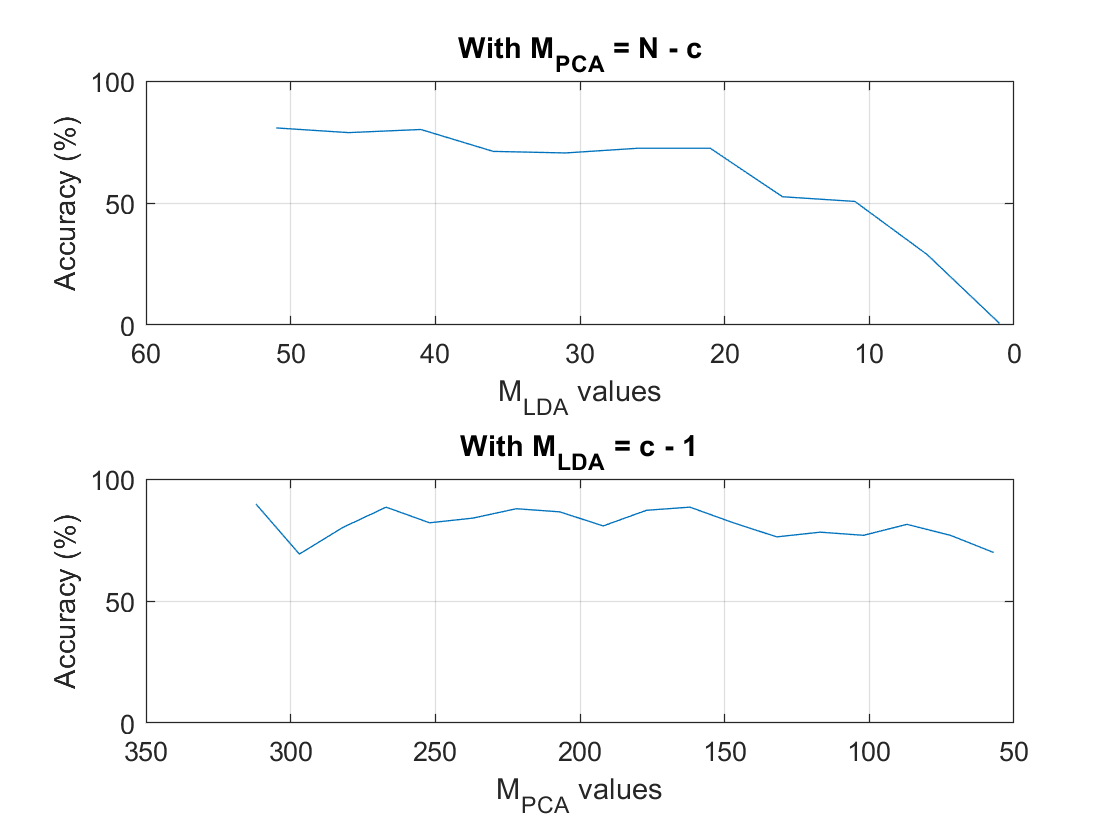
\includegraphics[width = \linewidth]{../results/ex2LDA/accuracy_vs_Ms.png}
    \caption{Model parameters vs accuracy}
    \label{fig:mod_params_vs_acc}
\end{figure}

\subsubsection{Ranks of the scatter matrices}
The scatter matrices are defined as sums of outer vector products, all of rank 1.
We confirm that the rank of the within-class-scatter matrix (Sw) is $N - c$. To obtain individual class scatter matrices, Si, we sum all the outer products of each class vector, from which the class mean was removed, with itself. Since the mean is a linear combination of the class vectors, we lose 1 rank in the Si matrix (rank $Ni - 1$, where Ni is the number of class vectors). The Sw matrix is the sum of all the Si matrices giving the rank $c(Ni - 1) = N - c$, where N is the total number of the training vectors.

The rank of the between-class-scatter matrix (Sb) is found to be $c - 1$, as expected. Sb is similarly obtained as a sum of matrices obtained from vector outer products with itself. Here, each class-mean vector has the global-mean vector removed, and then expanded into a matrix of rank 1. As before, the global-mean vector is a linear combination of class-mean vectors, which is why we lose one rank, and after summation we end up with the matrix of rank $c - 1$.

\subsubsection{Confusion matrix, Success and Failure cases}
The confusion matrix is presented in Figure \ref{fig:M_LDA_conf_mat}, with the example success cases in Figure \ref{fig:MLDA_success} and all the failure cases in Fingure \ref{fig:MLDA_fail}
Looking at the confusion matrix, it appears that there is larger miss-classification of certain classes compared to others. In this particular case, a lot of classes were miss-classified as class 3. The reference LDA coefficients are obtained by projecting the training images to the PCA subspace and then to the LDA subspace. With our training data split (70\%), this gives 7 reference coefficients per class. It's possible that, with the particular selection of training images for class 3, the reference coefficients of class 3 have greater scatter (and overlap with other classes) in the learned LDA subspace. Hence the NN classifier miss-classifies as class 3 more often.

\begin{figure}[htb!]
    \centering
    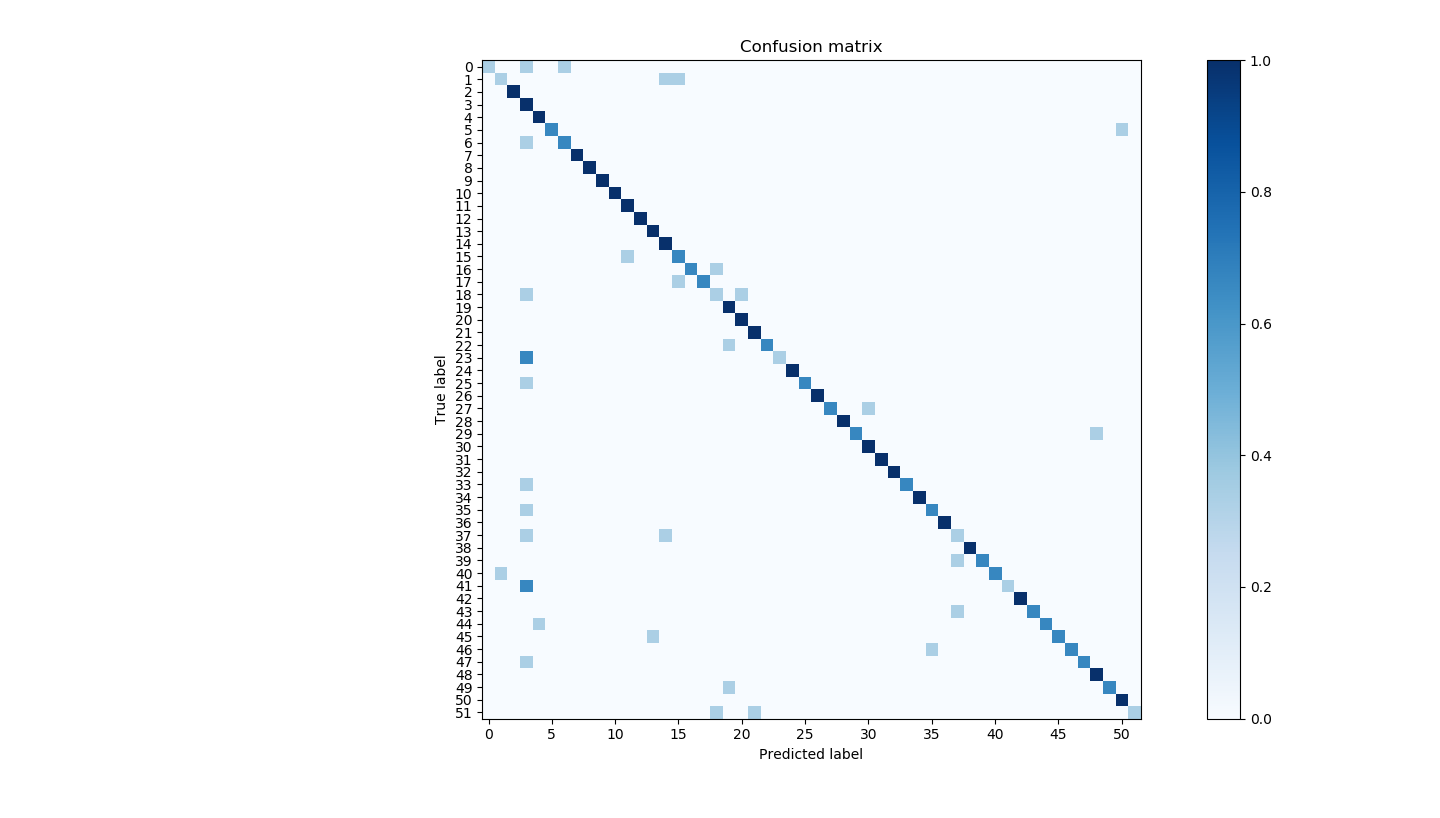
\includegraphics[width = \linewidth]{../results/ex2LDA/LDA_Conf_mat2.png}
    \caption{Confusion matrix}
    \label{fig:M_LDA_conf_mat}
\end{figure}

\begin{figure}[htb!]
    \centering
    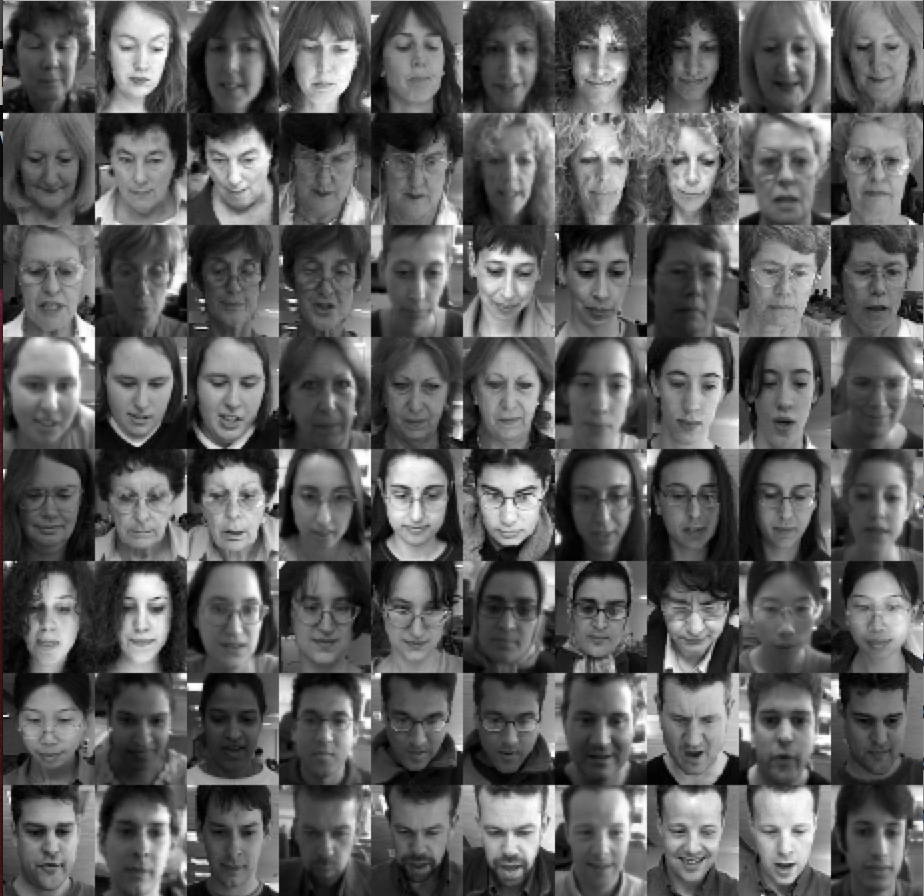
\includegraphics[width = \linewidth]{../results/ex2LDA/LDA_Example_Successes_crop.png}
    \caption{Example success cases}
    \label{fig:MLDA_success}
\end{figure}

\begin{figure}[htb!]
    \centering
    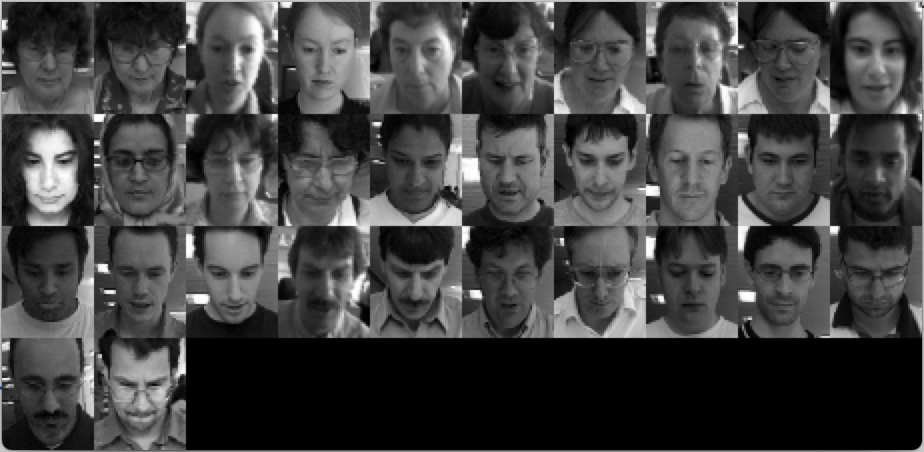
\includegraphics[width = \linewidth]{../results/ex2LDA/LDA_Example_Failiures.png}
    \caption{Fail cases}
    \label{fig:MLDA_fail}
\end{figure}

\subsection{PCA-LDA Ensemble}

Our model consisted of a number $T$ of sub-models made of one PCA unit,one following LDA unit and a nearest-neighbour classifier (NN). In each unit $t$, the PCA unit reduced the dimensionality of its input by applying the transform $W_{PCA}^t$, made of $M_{PCA}^t$ eigenfaces. The reduced data was then transformed by $W_{LDA}^t$, made of $M_{LDA}^t$ fisherfaces. The NN algorithm then assigns the resulting fisherfaces to their nearest neighbour. Each unit was trained sequentially, and their individual training data was used to reduce the training data and find the class-wise reference fisherfaces ($F_{c_i} \in \mathbb{R}^{D X W_{c_i}}$, where $W_{c_i}$ denotes the number of examples for the class $C_i$ in the training set).  By default, $M_{PCA}^t = N - c$ and $M_{LDA}^t = c - 1$. For each unit,  the cosine distance between the fisherfaces of the testing data and each of the vectors making up $F_{c_i}$ was calculated. Within a class, only the minimal distance was kept. All distances were then normalized and inverted, getting the probability distribution $p(x \in c_i)$ . The fusion of the unit outputs was chosen between 'mean', where the mean of the probability distribution between all units was taken and the minimal distance class was chosen, 'product', where instead of mean the product was taken, and 'majority', where each unit votes for there minimal distance class, and the class with the highest number of votes throughout the ensemble wins.

\subsubsection{Bagging}

The training data was randomised and split identically to Exercise 1. However, once the training data had been obtained, it was sampled into $T$ bags, by selecting a data point uniformly from the training dataset, with replacement. We denote the amount of data per bag with $n_t$. Using the product fusion rule, this bagging technique contributed to the randomness of each unit and thus their decorrelation, which will be investigated later. Figure \ref{fig:acc_vs_bag} highlights the gain in robustness that comes with bigger bag sizes. The repeated data percentage was found to be $37 \%$ for $n_t = N$, and $40 \%$ for $n_t = 450$. No significant changes were observed in terms of correlation.
\begin{figure}[htb!]
    \centering
    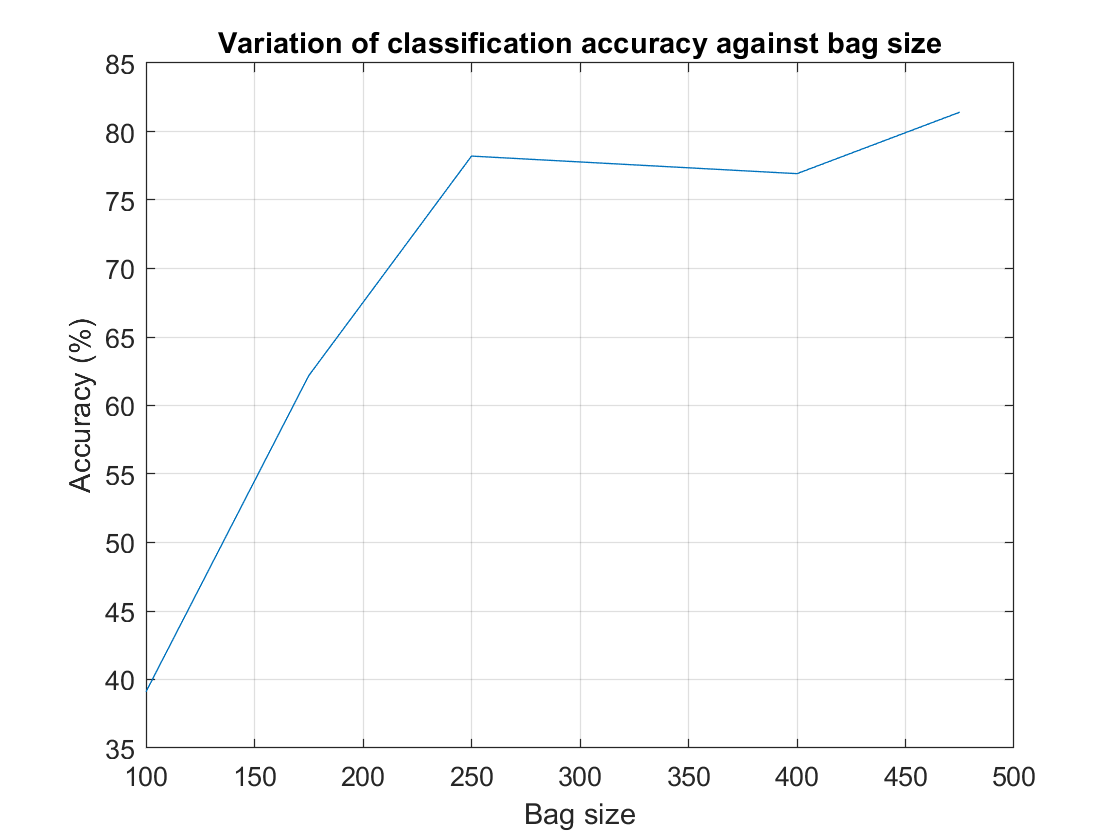
\includegraphics[width=\linewidth]{../results/ex2LDAEnsemble/acc_vs_bag_size.png}
    \caption{The bag size $n_t$ was equal for all units. (fusion : product, T=8, no randomisation of parameters}
    \label{fig:acc_vs_bag}
\end{figure}

A bag size of $n_t = 400$ was chosen as a default value for the remaining experiments.

\subsubsection{$M_{PCA}^t$ and $M_{LDA}^t$}:
The role of $M_{PCA}^t$ and $M_{LDA}^t$ was investigated by varying their value between 0 and their default value ($N - c$ and $c - 1$) and recording the classification accuracy over the testing data. The results, shown in Figure \ref{fig:mld_acc}, prove that the number of fisherfaces used for classification plays an important role in the discriminatory capability of the algorithm. The success rate quickly dropped as the fisherfaces became more sparse. Conversely, the number of eigenfaces plays a less important role: the classification accuracy experiences little change as the PCA subspace gets dimensionally reduced. As we have seen before in B), it seems as the LDA can deal with more sparse feature space equivalently well as with more dense feature spaces.


\begin{figure}[htb!]
    \centering
    \begin{subfigure}[b]{0.5\textwidth}
        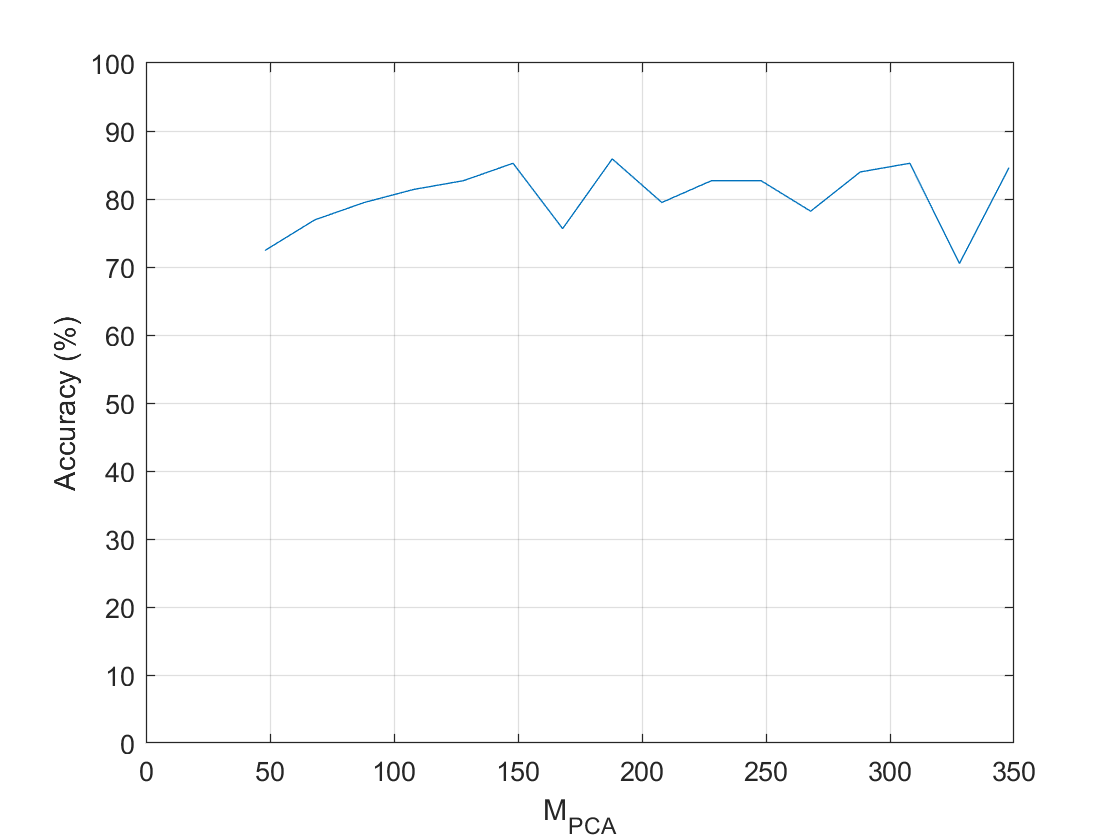
\includegraphics[width=\textwidth]{../results/ex2LDAEnsemble/acc_vs_mpca.png}
        \caption{Changing the $M_{PCA}$ values for all units simultaneously. Default value of 312. (fusion: product, T = 8, $n_t$ = 400,no randomisation of parameters)}
        
        \quad
    \end{subfigure}
    \begin{subfigure}[b]{0.5\textwidth}
        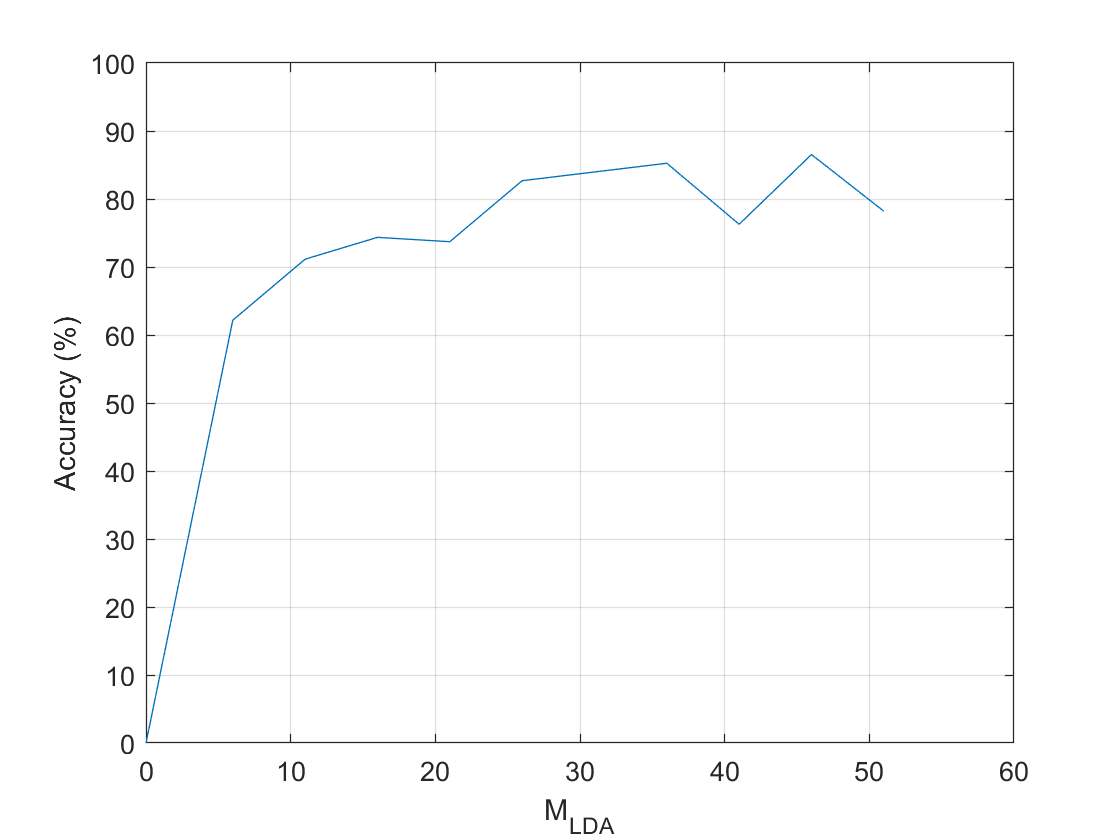
\includegraphics[width=\textwidth]{../results/ex2LDAEnsemble/acc_vs_mlda.png}
        \caption{Changing the $M_{LDA}$ values for all units simultaneously. Default value of 51. (fusion: product, T = 8, $n_t$ = 400, no randomisation of parameters)}
        
        \quad
    \end{subfigure}
    \caption{Evolution of classification accuracy when changing the model parameters}
    \label{fig:mld_acc}
\end{figure}

\subsubsection{Randomness and correlation}
We generated three different models, using the default parameters ($T = 8, n_t = 400$). In Figure \ref{fig:corrs}, the leftmost model was generated without using bagging (so using a fixed training data), and with default $M_{LDA}$ and $M_{PCA}$ values. As expected, all 8 units are fully correlated. We then introduce a first element of randomness by randomising $M_{LDA}$ and $M_{PCA}$ uniformly between a fourth of their default value and their default value (parameter randomisation), leading to the second correlation matrix. Finally, we add bagging to the algorithm and get the strongly decorrelated model, represented by the third correlation matrix.  

\begin{figure}[htb!]
    \centering
    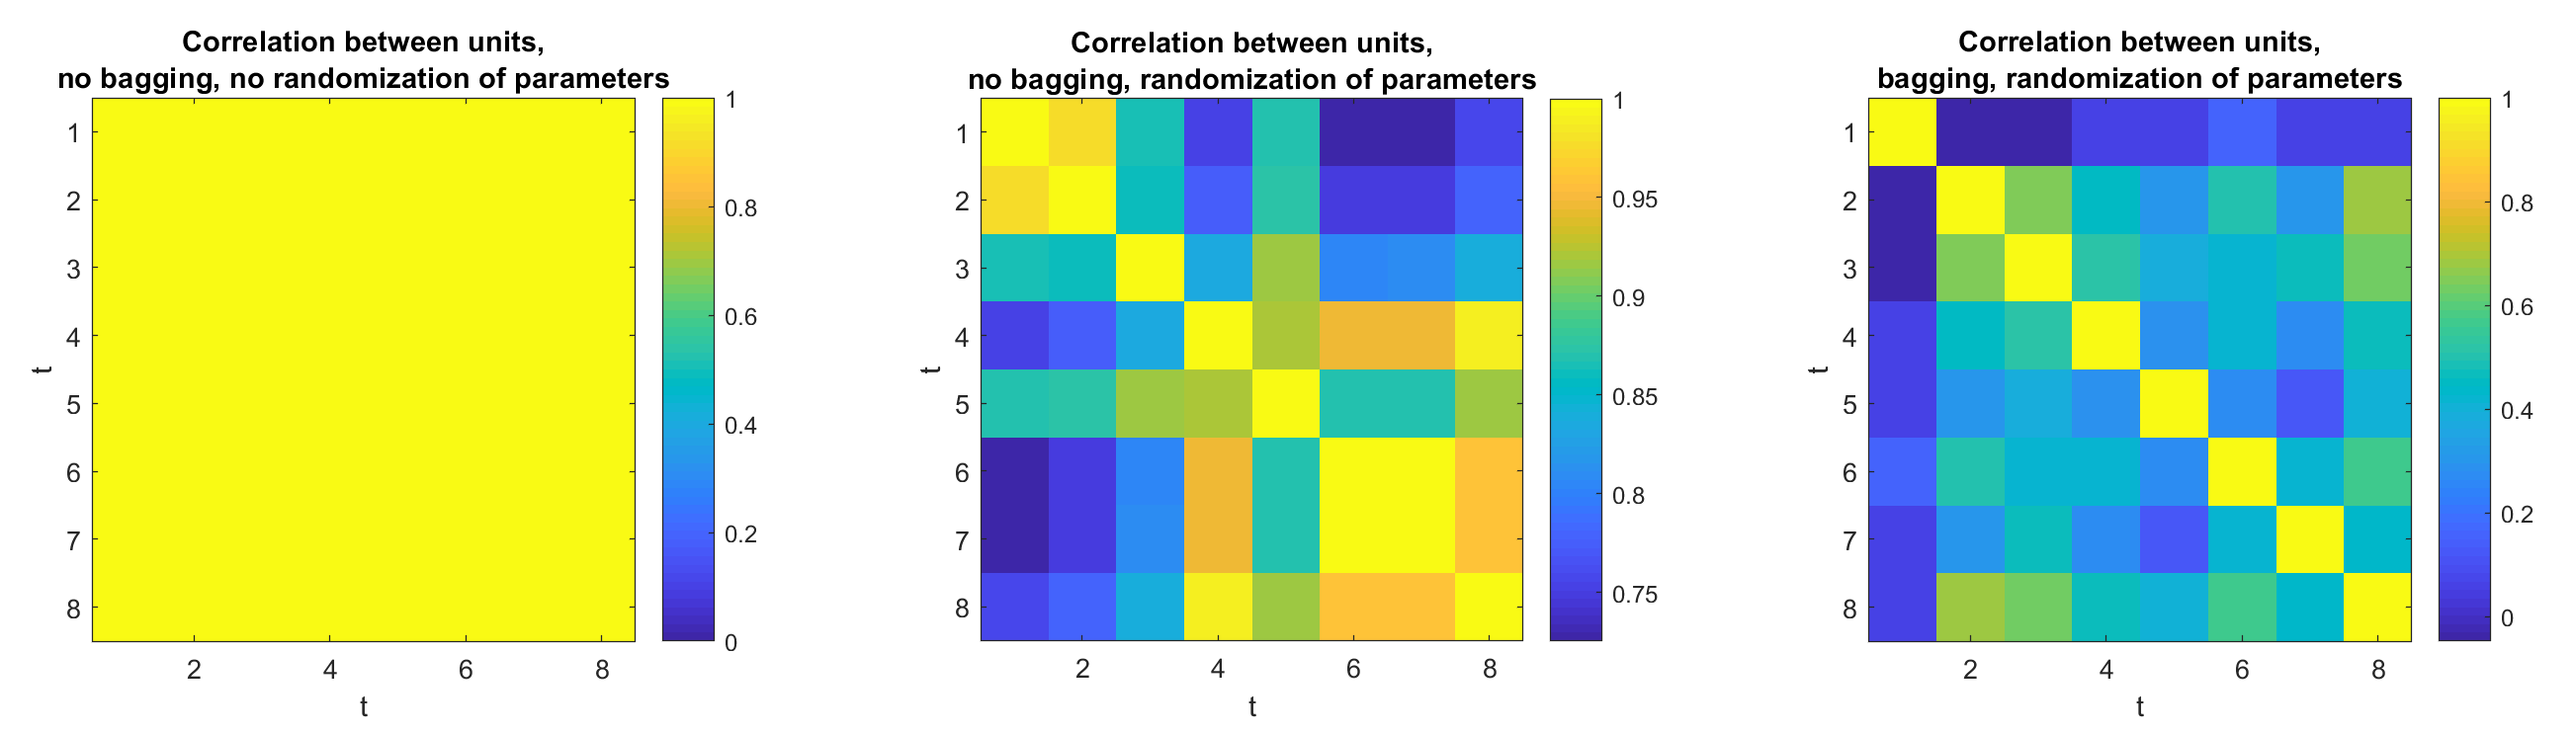
\includegraphics[width=\linewidth]{../results/ex2LDAEnsemble/correlation.png}
    \caption{Correlation matrix between the units. $T = 8$. The more randomness is introduced to the model, the more decorrelated the model (from left to right). (fusion: product, T = 8, $n_t$ = 400)}
    \label{fig:corrs}
\end{figure}

\subsubsection{Confusion and classification performance}
The performance of the different fusion rules was tested and plotted in Figure \ref{fig:conf_matrix_ensemble} and \ref{fig:acc_unit_error}, with bagging enabled, and parameter randomisation enabled for Figure \ref{fig:conf_matrix_ensemble}. In Figure \ref{fig:acc_unit_error}, the parameter randomisation was alternatively enabled/disabled. When randomisation was enabled, the majority voting rule performed better than both product and mean rules, which both performed equally well. Because of the randomness introduced to the units, it is understandable how the product and mean fusion rules performed less well as they are more susceptible to noise. However, when randomisation was disabled, the product fusion rule proved to perform the best, since the unit outputs were more similar and would be amplified by multiplication. These figures also show that randomness makes the ensemble perform better, making it more robust.
\begin{figure}
    \centering
    \begin{subfigure}[b]{0.3\textwidth}
        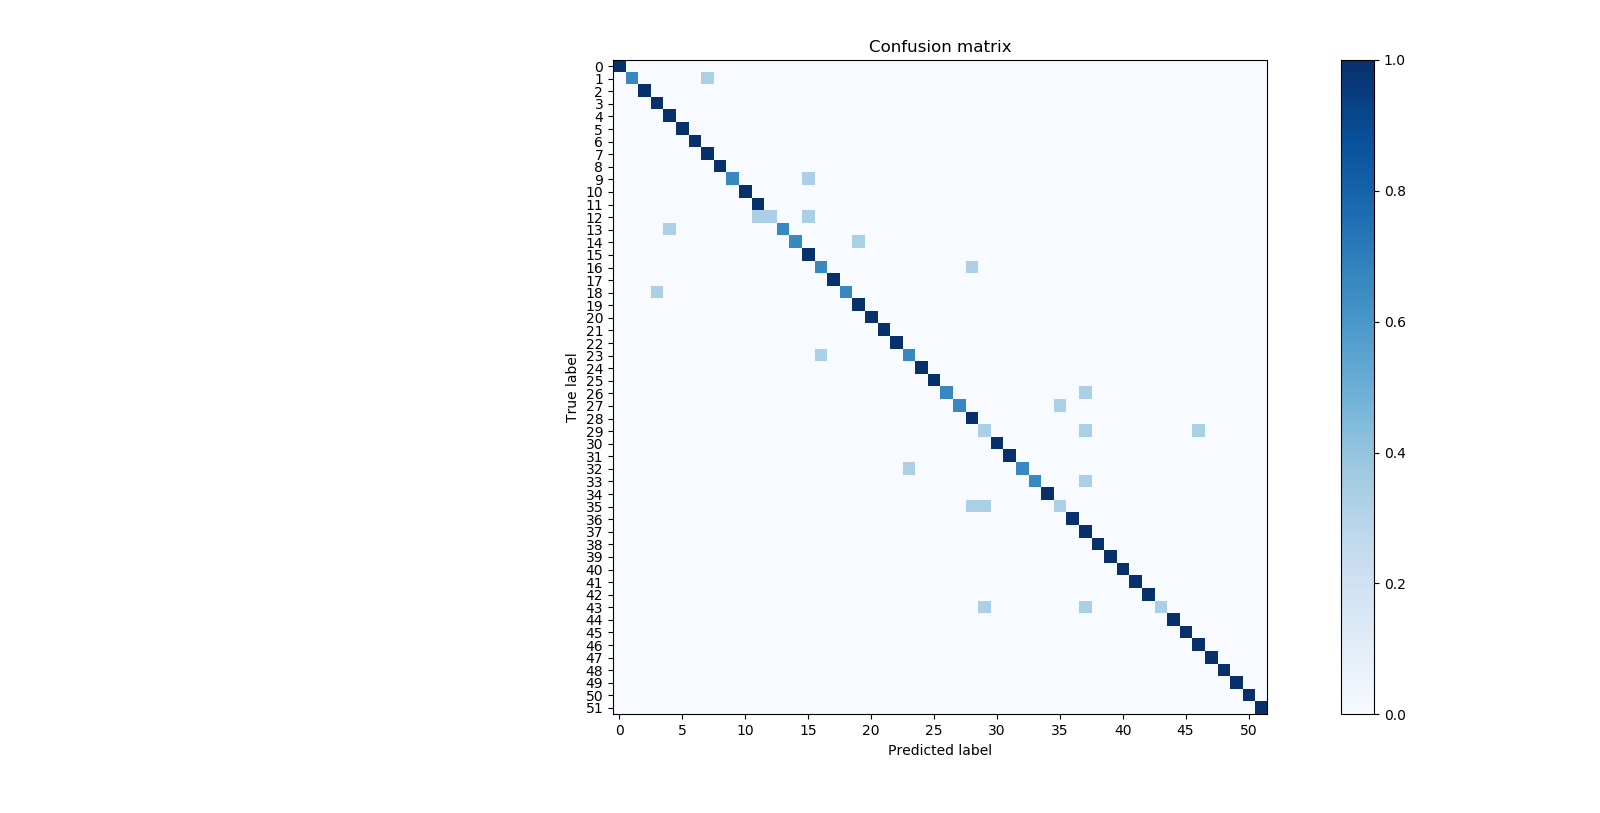
\includegraphics[width=\textwidth]{../results/ex2LDAEnsemble/conf_matrix_rand_mean.png}
        \caption{Mean fusion. Overall accuracy: 87.2 \% }
    \end{subfigure}    
    \begin{subfigure}[b]{0.3\textwidth}
        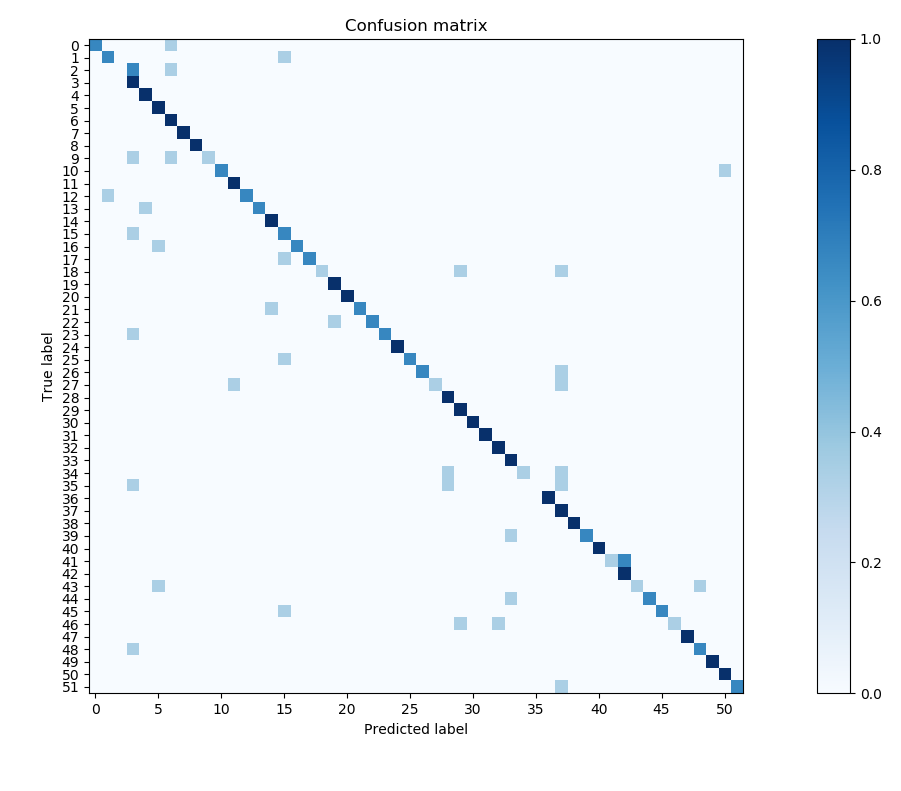
\includegraphics[width=\textwidth]{../results/ex2LDAEnsemble/conf_matrix_rand.png}
        \caption{Product fusion. Overall accuracy: 87.8 \%}
    \end{subfigure}  
    \begin{subfigure}[b]{0.3\textwidth}
        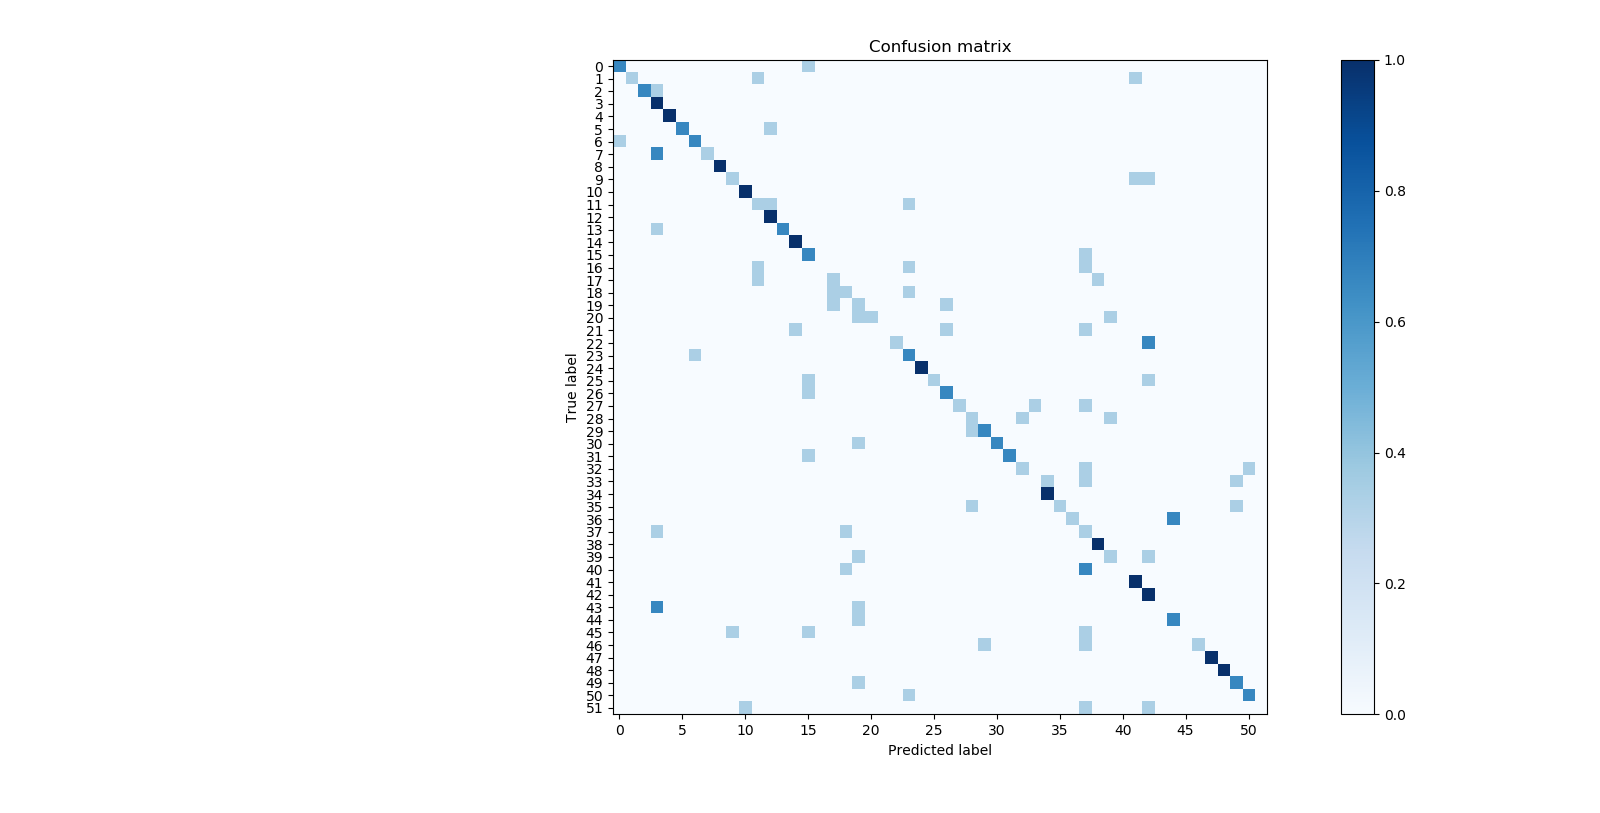
\includegraphics[width=\textwidth]{../results/ex2LDAEnsemble/all_rand_maj_conf.png}
        \caption{Majority voting fusion. Overall accuracy: 90.0\%}
    \end{subfigure}    
    
    \caption{Confusion matrices for different fusion rules, T=8, $n_t = 400$, randomisation of parameters}
    \label{fig:conf_matrix_ensemble}
    
\end{figure}
\begin{figure}
    \centering
    \begin{subfigure}[b]{0.5\textwidth}
        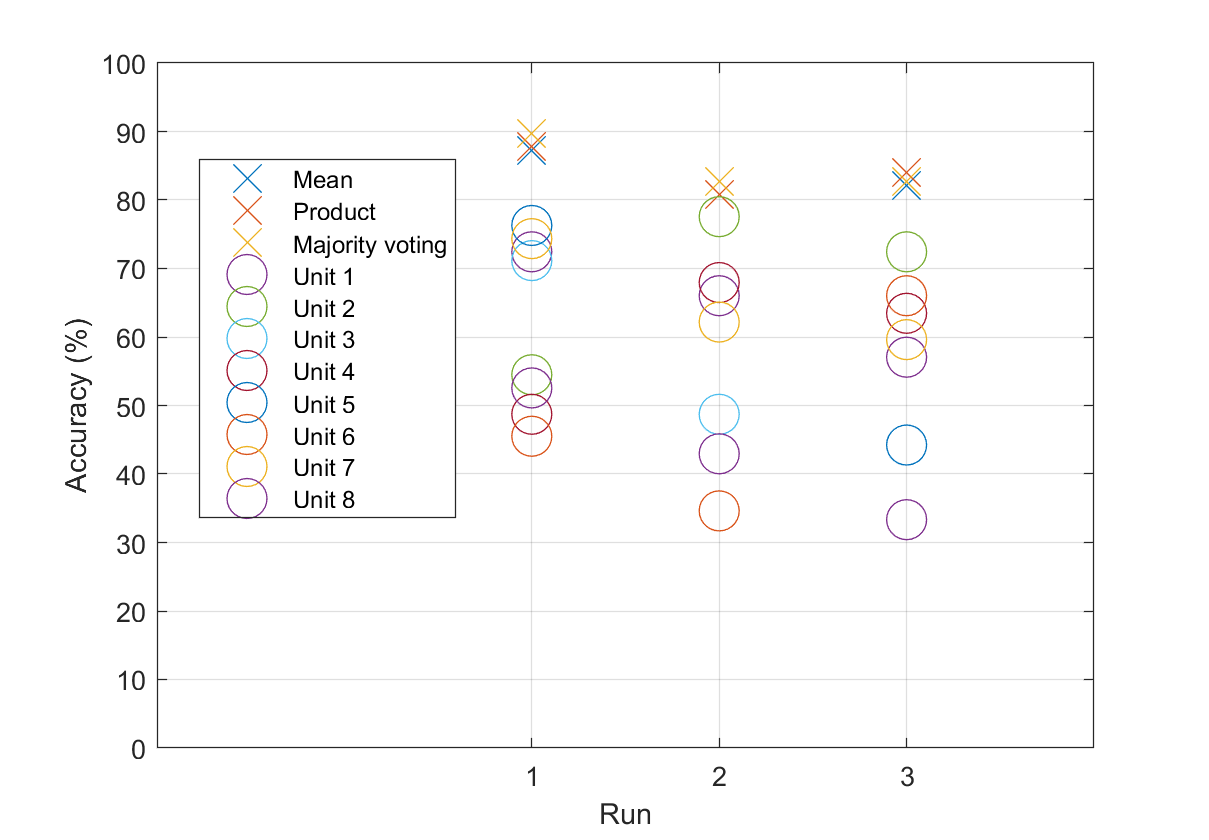
\includegraphics[width=\linewidth]{../results/ex2LDAEnsemble/acc_vs_unit.png}
        \caption{Parameter randomisation enabled}
    \end{subfigure}
    \begin{subfigure}[b]{0.5\textwidth}
        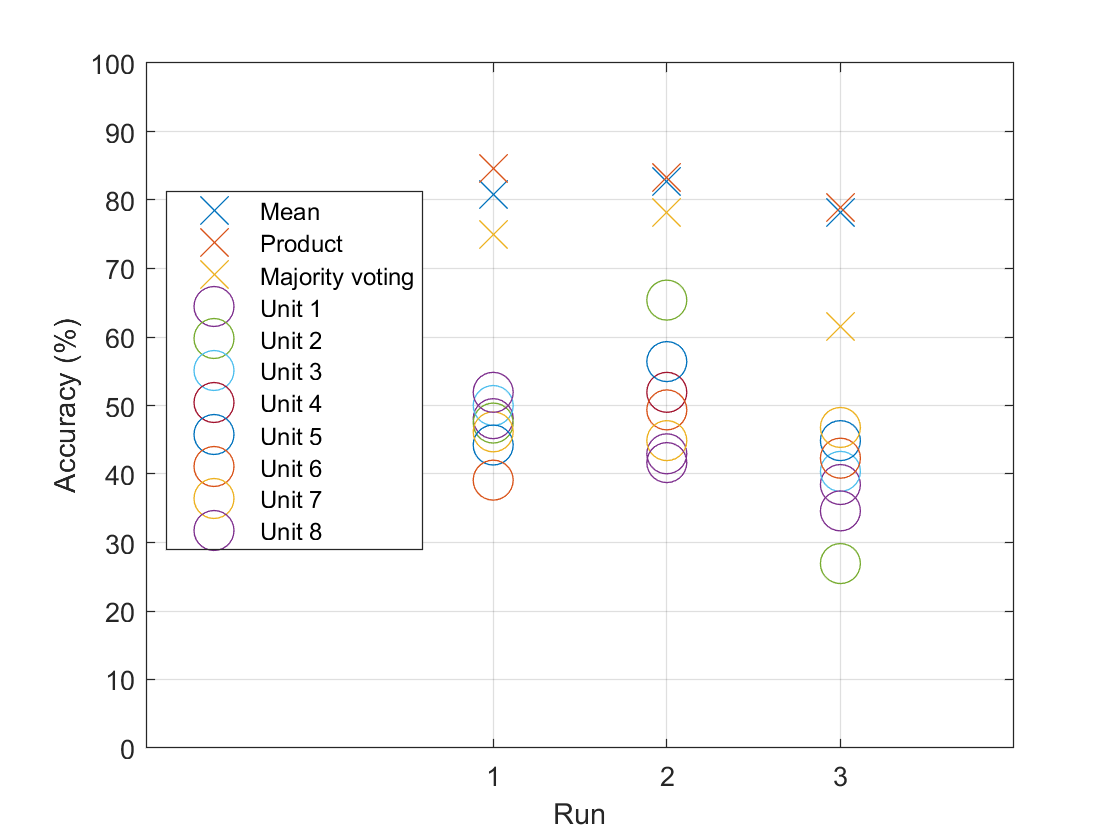
\includegraphics[width=\linewidth]{../results/ex2LDAEnsemble/acc_vs_unit_no_rand.png}
        \caption{Parameter randomisation disabled}
    \end{subfigure}
    \caption{Individual unit accuracy and global classification accuracy of the different fusion rules over three different training runs. (T = 8 $n_t = 400$, parameter randomisation enabled/disabled)}
    \label{fig:acc_unit_error}
\end{figure}

\subsubsection{Influence of number of units}
The effect of varying the number of units in the ensemble is shown in Figure \ref{fig:acc_vs_n_units} and \ref{fig:acc_vs_n_units_rand}. We can see that while increasing the number of units always has a positive impact on the classification performance with no randomisation, randomising the parameters makes the ensemble converge to an efficient point faster, with a lower number of units required. 

\begin{figure}

    \centering
    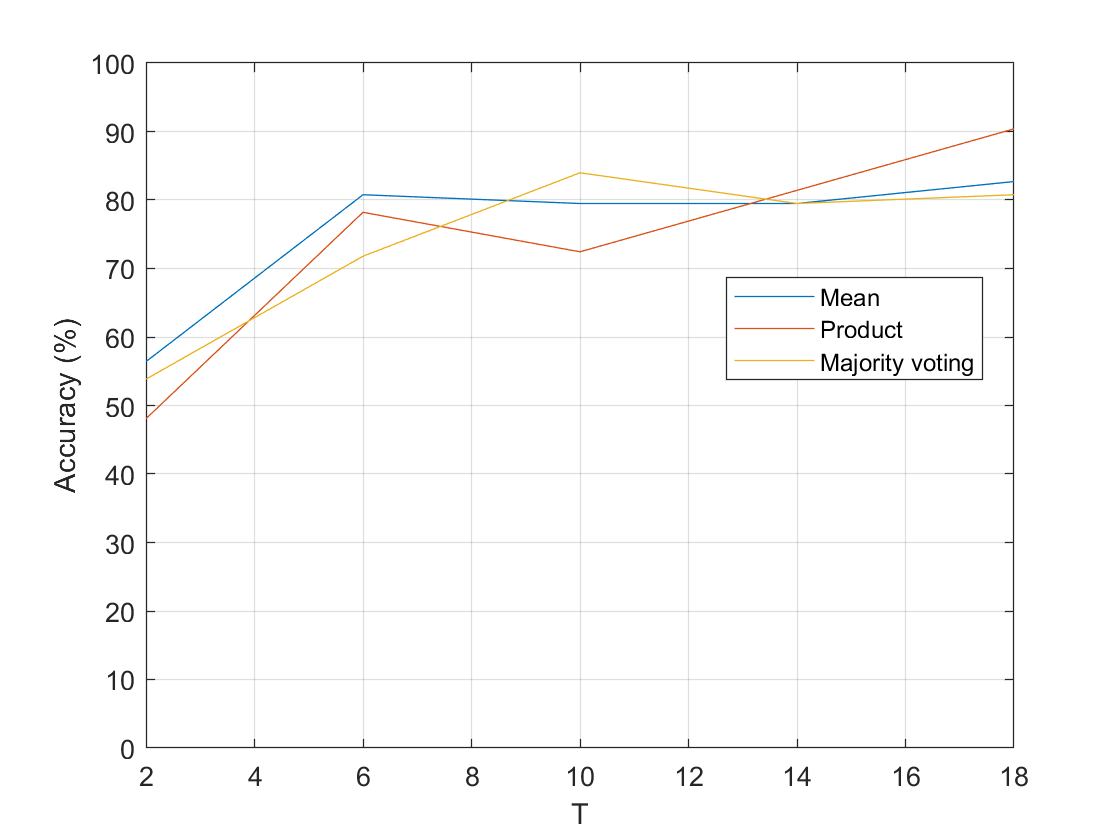
\includegraphics[width=\linewidth]{../results/ex2LDAEnsemble/acc_vs_n_unit.png}
    \caption{Accuracy of classification against number of units used. ($n_t = 400$, no parameter randomisation }
    \label{fig:acc_vs_n_units}
\end{figure}
\begin{figure}
    \centering
    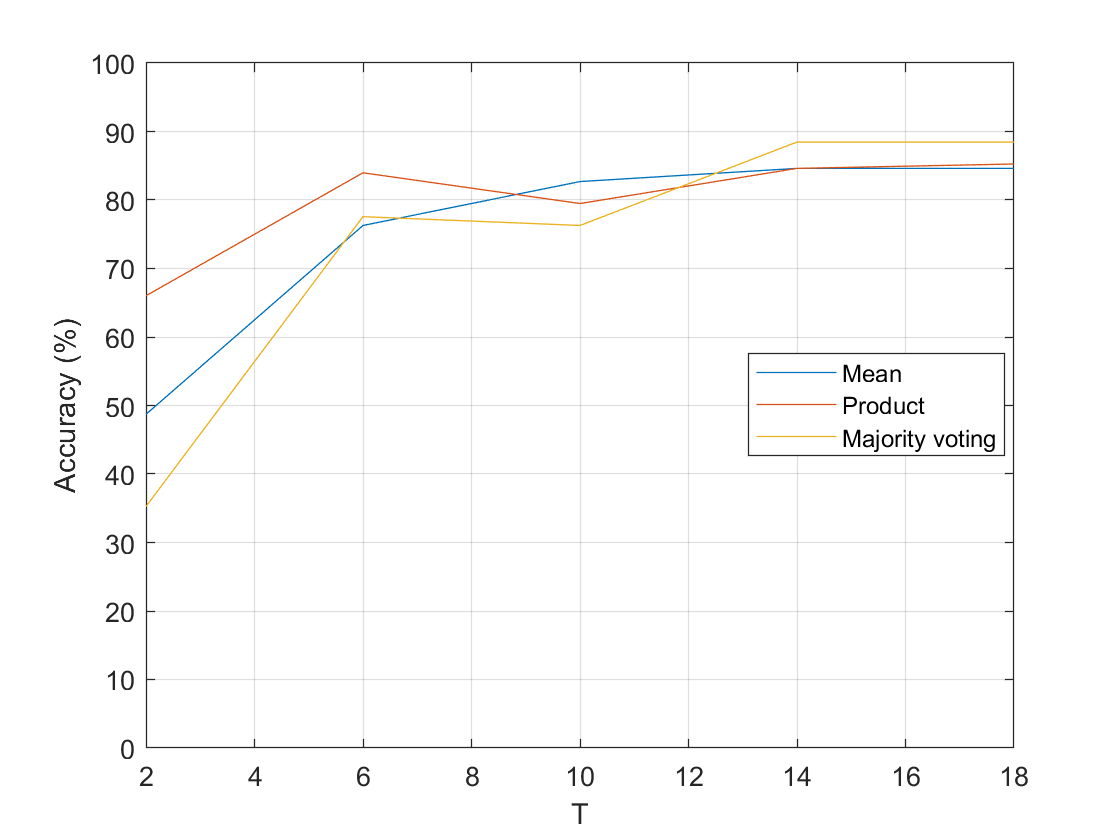
\includegraphics[width=\linewidth]{../results/ex2LDAEnsemble/acc_vs_n_unit_rand.png}
    \caption{Accuracy of classification against number of units used. ($n_t = 400$, with parameter randomisation }
    \label{fig:acc_vs_n_units_rand}
\end{figure}


\section{Appendix}
\begin{figure}[htb!]
    \centering
    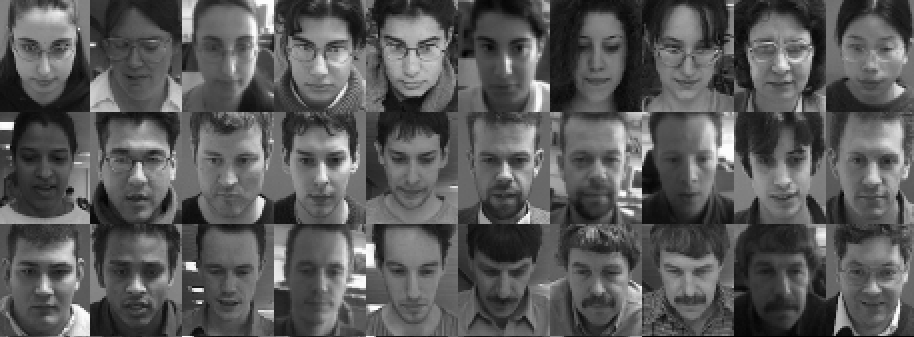
\includegraphics[width=\linewidth]{../results/1bb/NN_FAIL2_cropped.png}
    \caption{NN Classification Fail Cases}
    \label{fig:nn_fails}
\end{figure}

\begin{figure}[htb!]
    \centering
    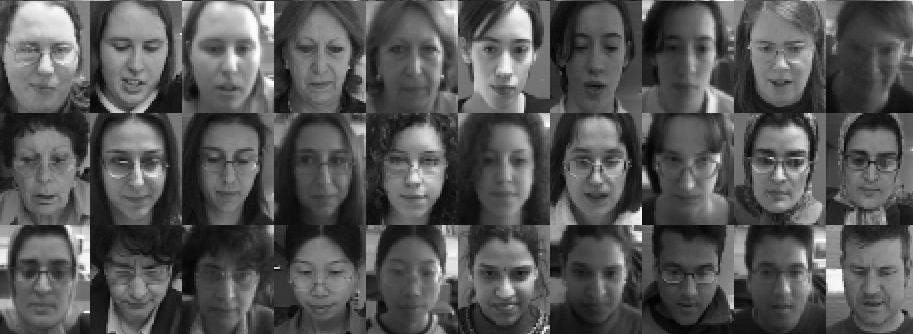
\includegraphics[width=\linewidth]{../results/1bb/NN_SUCCESS2_cropped.png}
    \caption{NN Classification Success Cases}
    \label{fig:nn_successes}
\end{figure}

\begin{figure}[htb!]
    \centering
    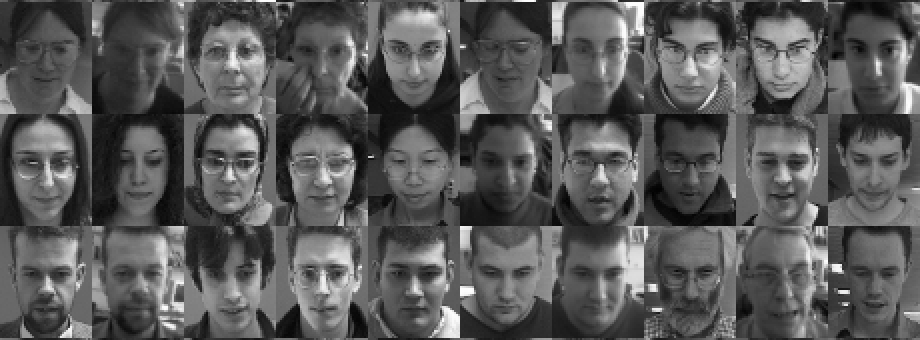
\includegraphics[width=\linewidth]{../results/1bb/REC_FAIL2_cropped.png}
    \caption{Classification by Reconstruction Fail Cases}
    \label{fig:rec_fails}
\end{figure}

\begin{figure}[htb!]
    \centering
    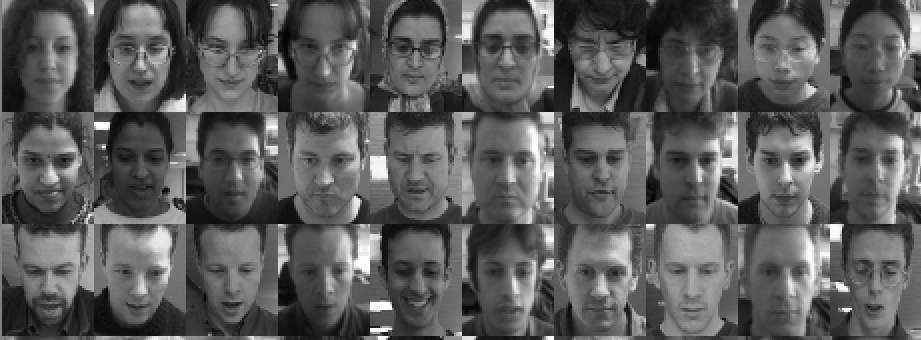
\includegraphics[width=\linewidth]{../results/1bb/REC_SUCCESS2_cropped.png}
    \caption{Classification by Reconstruction Success Cases}
    \label{fig:rec_successes}
\end{figure}
\end{document}